\subsection{Overview of the architecture}
Tinker system has to deal with challenges at different levels from hardware interface to artificial intelligence. Thus, a multi-level, distributed architecture based on ROS is employed to meet such requirement. The hardware layer are the motors and the sensors of the robot. The hardware-communication layer is responsible for controlling the motors and acquiring information from the sensors. The output of the hardware layer is ROS-compatible sensor images including camera image, point cloud and multiple other topics. The logic layer is responsible for providing basic functions of a robot such as manipulation, navigation, human tracking, object recognition, speech recognition and synthesis etc. The decision layer listens to topics published by the logic layer and makes decision for the next high-level action to make.
\subsubsection{The hardware layer}

The motors we use are:
\begin{enumerate}
    \item Times Brilliant DMS-055A motors for driving the chassis and the platform
    \item ALFS ASME-03 high-torque servo for the robot arm
    \item Dynamixel MX-64 servo for robot hand
\end{enumerate}
The sensors we use are:
\begin{enumerate}
    \item Hokuyo URG04LX laser scanner for navigation
    \item Kinect v2 depth camera for navigation and object detection
    \item Logitech C170 camera for object recognition and detection
    \item Infrared proximity sensor for manipulation
\end{enumerate}
\subsubsection{The hardware-communication layer}
The hardware communication layer must be highly scalable to quickly install and remove different sensors and executors. All control commands of the robot are sent to the ROS nodes running on the Xilinx ZYNQ soc. The ZYNQ soc then controls the motor peripheral. 
For sensors, those which already have had a ROS wrap like Kinect, camera and laser scanner are directy connected to the laptop computer while the feedback of motors other senor messages that need further processing to ROS messgaes are sent to ZYNQ, where ROS nodes are running to collect information and tranlate them to ROS messages.
\begin{figure}[!t]
	\centering
    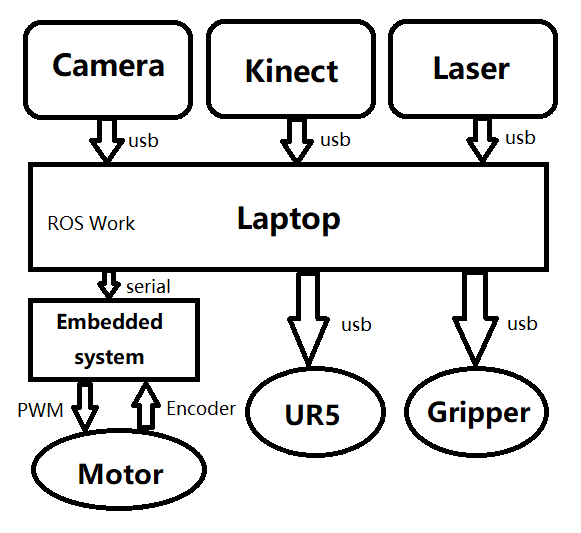
\includegraphics[scale=0.5]{commuication_arch.png}
    \caption{The architecture of the hardware-communication layer}
    \label{arch_comm}
\end{figure}

\subsubsection{The logic layer}
Most important robot functions are implemented in this layer. The main components in this layer include:
\begin{enumerate}
    \item Navigation: Mapping, localization, route-planning and collision avoidance
    \item Vision: Human recognition, object recognition and their tracking.
    \item Speech: Speech recognition and synthesis
    \item Arm control: Manipulation with feedback from vision
\end{enumerate}

\subsubsection{The decision layer}
Task planning is done in decision layer. For different tasks, modules in decision layer run as state machine. They integrate different information from the low layer to judge the state they are in and then give different orders or make different responses. Each module deal with a single task, sharing the common information from the lower layers.

